\documentclass[a4paper, 12pt]{article}

%\usepackage{cmap}
\usepackage[T2A]{fontenc}
\usepackage[utf8]{inputenc}
\usepackage[english, russian]{babel}
\usepackage{graphicx}
\usepackage[top=1in, bottom=1in, left=3.2cm, right=2.6cm]{geometry}
\graphicspath{./}
\usepackage{biblatex}
\addbibresource{lib.bib}
\linespread{1.5}
\usepackage{ragged2e}
\justifying
\usepackage{listings}
\usepackage{color}
\usepackage{amsmath}
\newcommand{\eqdef}{\stackrel{\mathrm{def}}{=}}

\begin{document}
	
\begin{titlepage}
	\fontsize{12pt}{12pt}\selectfont
	\begin{figure}[t!]
		\centering
		
\includegraphics[scale=0.8]{bmstu}
	\end{figure}
	
	\noindent\rule{15cm}{3pt}
	\newline\newline
	\noindent 
	ФАКУЛЬТЕТ 
	\underline{«Информатика и системы управления»} \newline\newline
	
	\noindent КАФЕДРА \underline{«Программное обеспечение ЭВМ и информационные технологии»}\newline\newline\newline\newline
	
	\centering {\Large Отчет по лабораторной работе № 2}
	\vspace{1mm}
	
	\centering {\Large По курсу: "Математическое моделирование"
		\vspace{8mm}	
		
		\centering \bf Программно-алгоритмическая реализация методаРунге-Кутта 4-го порядка точности при решении  системы ОДУ в задаче Коши.}
	\vspace{15mm}
	
	
	\begin{flushleft}
		{\large Студент: Турсунов Жасурбек Рустамович \\ Группа: ИУ7-66Б
			\\Оценка(баллы):
			\vspace{3mm}
			\\Преподователь: Градов Владимир Михайлович }
	\end{flushleft}
	
	\begin{center}
		\vfill
		Москва, \the\year
		~г.
	\end{center}
\end{titlepage}

\tableofcontents
\clearpage
\newpage

\section*{Введение}
\addcontentsline{toc}{section}{Введение}

	\textbf{Цель работы:} Получение навыков разработки  алгоритмов решения задачи Коши при реализации моделей, построенных на системе ОДУ, с использованием методов Рунге-Кутта 4-го порядка точности.
 
	

\clearpage
\newpage
\section{Аналитическая часть}
	\textbf{Исходные данные:} Задана система электротехнических уравнений, описывающих разрядный контур, включающий постоянное активное сопротивление $R_k$, нелинейное сопротивление $R_p (I)$, зависящее от тока $I$,  индуктивность $L_k$и емкость $C_k$.
	
	\begin{equation*} 
		\begin{cases}
			
			\frac{dI}{dT} = \frac{U -(R_k + R_p(I))I }{L_k}\\
			\Large \frac{dU}{dt} = - \frac{I}{C_k}
		\end{cases}
	\end{equation*}
	\\Начальные условия: $t = 0, I = I_0, U = U_0$.
	\\$I, U$- ток и напряжение на конденсаторе.
	\\Сопротивление $R_p$ рассчитать по формуле
	
	 \vspace*{1cm} \hspace*{3cm}\text{\Large $R_p = \frac{l_p}{2\pi R^2\int_0^1 \sigma(T(z))zdz}$}
	\vspace*{1cm} \\ Для функции $T(z)$ применить выражение $T(z) = T_0 + (T_w - T_0 ) z^m$. 
	\\Параметры  $T_0$, m находятся интерполяцией из таблицы 1 при известном токе $I$.
	\\Коэффициент электропроводности $\sigma(T)$ зависит от $T$ и рассчитывается интерполяцией из  таблицы 2.
	\\Таблица 1:\\
	\vspace*{10mm}\hspace*{40mm}\begin{tabular}{ | l | l | l | }
		\hline
		\textbf{$I, A$}& \textbf{$T_0$} & \textbf{m} \\ \hline
		0.5 & 6730 & 0.5\\ \hline
		1 & 6790 & 0.55\\ \hline
		5 & 7150 & 1.7\\ \hline
		10 & 7270 & 3\\ \hline
		50 & 8010 & 11\\ \hline
		200 & 9185 & 32\\ \hline
		400 & 10010 & 40\\ \hline
		800 & 11140 & 41\\ \hline
		1200 & 12010 & 39\\ \hline
	\end{tabular}
	
\clearpage
\newpage
	Таблица 2\\
	\vspace*{10mm}\hspace*{40mm}\begin{tabular}{ | l | l | l | }
	\hline
	\textbf{$T, K$}& \textbf{$\sigma, \frac{1}{Om cm}$} \\ \hline
	4000 & 0.031 \\ \hline
	5000 & 0.27 \\ \hline
	6000 & 2.05 \\ \hline
	7000 & 6.06 \\ \hline
	8000 & 12.0 \\ \hline
	9000 & 19.9 \\ \hline
	10000 & 29.6 \\ \hline
	11000 & 41.1 \\ \hline
	12000 & 54.1 \\ \hline
	13000 & 67.7 \\ \hline
	14000 & 81.5 \\ \hline
\end{tabular}

\vspace*{10mm} \hspace*{-7mm}Параметры разрядного контура:
\\$R$ = 0.35 см
\\$l_{э}$ = 12 см
\\$L_k$ = 187*10-6 Гн
\\$C_k$ = 268*10-6 Ф
\\$R_k$ = 0.25 Ом
\\$U_{co}$ = 1400 В
\\$I_o$ = 0..3 A
\\$T_w$ = 2000 K

\clearpage
\newpage
\section{Технологическая часть}

	\subsection{Листинг кода}
	\definecolor{codegreen}{rgb}{0,0.6,0}
	\definecolor{codegray}{rgb}{0.5,0.5,0.5}
	\definecolor{codepurple}{rgb}{0.58,0,0.82}
	\definecolor{backcolour}{rgb}{0.95,0.95,0.92}

	\lstdefinestyle{mystyle}{
		backgroundcolor=\color{backcolour},   
		commentstyle=\color{codegreen},
		keywordstyle=\color{magenta},
		numberstyle=\tiny\color{codegray},
		stringstyle=\color{codepurple},
		basicstyle=\ttfamily\footnotesize,
		breakatwhitespace=false,         
		breaklines=false,                 
		captionpos=b,                    
		keepspaces=true,                 
		numbers=left,                    
		numbersep=5pt,                  
		showspaces=false,                
		showstringspaces=false,
		showtabs=false,                  
		tabsize=4
	}

	\lstset{style=mystyle}

	\begin{lstlisting}[language=Python]
def interpolate(x, masX, masY):
		order = 1
		s = InterpolatedUnivariateSpline(masX, masY, k=order)
		return float(s(x))

def T(z):
	return (Tw - T0) * z**m + T0

def sigma(T):
	return interpolate(T, masT, masSigm)

def Rp(I):
	global m
	global T0
	m = interpolate(I, masI, masm)
	T0 = interpolate(I, masI, masT0)

	def func(z): return sigma(T(z)) * z
	integral = integrate.quad(func, 0, 1)
	Rp = le/(2 * numpy.pi * R**2 * integral[0])

	return Rp

def f(xn, yn, zn):
	return -((Rk + m_Rp_global) * yn - zn)/Lk

def phi(xn, yn, zn):
	return -yn/Ck

def fourth_order(xn, yn, zn, hn, m_Rp):
	global m_Rp_global
	m_Rp_global = m_Rp

	k1 = hn * f(xn, yn, zn)
	q1 = hn * phi(xn, yn, zn)

	k2 = hn * f(xn + hn/2, yn + k1/2, zn + q1/2)
	q2 = hn * phi(xn + hn/2, yn + k1/2, zn + q1/2)

	k3 = hn * f(xn + hn/2, yn + k2/2, zn + q2/2)
	q3 = hn * phi(xn + hn/2, yn + k2/2, zn + q2/2)

	k4 = hn * f(xn + hn, yn + k3, zn + q3)
	q4 = hn * phi(xn + hn, yn + k3, zn + q3)

	yn_1 = yn + (k1 + 2*k2 + 2*k3 + k4)/6
	zn_1 = zn + (q1 + 2*q2 + 2*q3 + q4)/6

	return yn_1, zn_1
	\end{lstlisting}

	
\clearpage
\newpage
\section{Исследовательская часть }

	
	\subsection{Примеры работы}
	Графики зависимости от времени импльса t: $I(t), U(t), R_p (t), I(t) * R_p (t), T_0 (t)$ при заданных выше параметрах:
	\begin{figure}[h]
		\centering 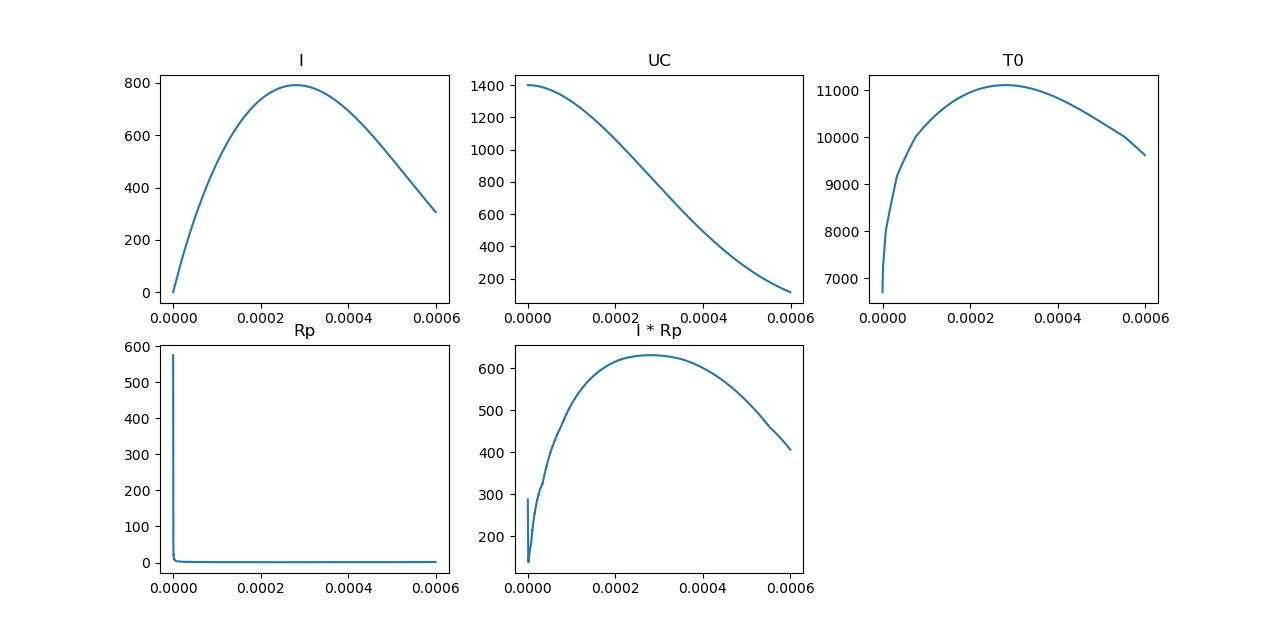
\includegraphics[scale=0.5]{1}
	\end{figure}
	

    График зависимости $I(t)$при $R_k + R_p = 0$.
	\begin{figure}[h]
		\centering
		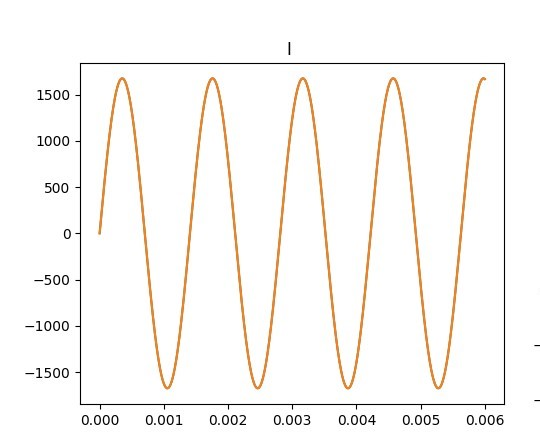
\includegraphics[scale=0.6]{2}
	\end{figure}
	\\Так как сопротивление в контуре нулевое, контур - колебательный, и колебания тока не затухают.
\clearpage
\newpage
	График зависимости $I(t)$ при $R_k + R_p = 200$ Ом в интервале значений t0-20 мкс.
	\begin{figure}[h]
		\centering
		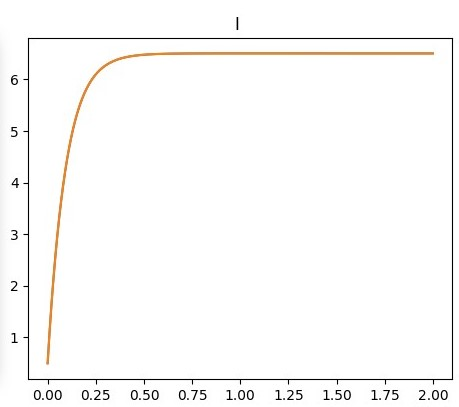
\includegraphics[scale=0.6]{3}
	\end{figure}
\section{Ответы на вопросы}
\textbf{1) Какие способы тестирования программы можно предложить?}
\\При тестировании программы изменять шаг.  Уменьшая шаг, мы дойдем до момента, когда новое уменьшение шага никак не изменит полученный результат. Отсюда следует, что полученный результат является точным. 
Также при тестировании нужно учесть, что работа моделируемого электрического контура описывается теоретически законами физики. Поэтому проверяются ситуации, когда сопротивление в контуре нулевое ,и он становится колебательным, а также когда сопротивление наоборот велико.

\textbf{2) Из каких соображений проводится выбор того или иного метода, учитывая, что чем выше порядок точности метода, тем он более сложен?}
\\ Выбор метода проводится с учетом точности и шага. При большом шаге для получения достаточно точного результата лучше использовать методы более высокого порядка точности. Сложность вычислений на каждой итерации в таком случае будет компенсирована тем, что самих итераций при большом шаге будет меньше. При маленьком шаге методы менее высокого порядка точности дают такой же результат, как и методы более высокого порядка, для которых количество вычислений значительно больше. Также стоит учесть, что количество итераций при маленьком шаге возрастает. Поэтому в этом случае лучше выбрать методы менее высокого порядка точности.
\\ \textbf{3) Получите систему разностных уравнений для решения сформулированной задачи неявным методом трапеций. Опишите  алгоритм реализации полученных уравнений.}
\\Неявный метод трапеций – это метод Рунге-Кутта второго порядка точности с $\alpha$ = 0.5
\\  Уравнение \\\text{\Large $y_{n+1} = y_n + h_n[(1 - \alpha) f(x_n, y_n) + f(x_n + \frac{h}{2\alpha}, y_n + \frac{h}{2\alpha}f(x_n, y_n))]$} 
\\ \\сводится к уравнению \text{\Large $y_{n+1} = y_n + h_n[\frac{f(x_n, y_n) + f(x_n, h, y_n + hf(x_n, y_n))}{2}]$}

\hspace*{-6mm}Получаем систему разностных уравнений:
\begin{equation*} 
	\begin{cases}
		
		I_{n+1} = I_n + h_n[\frac{f(I_n, U_{cn} + f(I_n + h, U_{cn} + hg(I_n)))}{den}]\\
		U_{c_{n+1}} = U_{cn} + h_n[\frac{g(I_n) + g(I_n + h)}{2}]
	\end{cases}
\end{equation*}
Имеется исходная система:
\begin{equation*} 
	\begin{cases}
		
		I^{'(t)} = \frac{U_c - I(R_k + R_p)}{L_k}\eqdef f(I, U_c)\\
		U'(t) = -\frac{I}{C_k} \eqdef (g(I)) \\
		I(0) = I_0 \\
		U(0) = U_{c0}
	\end{cases}
\end{equation*}

Подставляя уравнения производных в разностные уравнения, можно найти решение итерационно, так как на i-м ходу известны $I_i, U_{ci}, h_i$.
Подставив их в полученные формулы, находим $I_{i+1} и U_{c_{i+1}}, h_{i+1}$ известно заранее (например, шаг может быть постоянным).

 
\end{document}